\section{Loom: Physical Storage Layout Compilation}
\label{sec:loom}

\begin{figure*}[t]
\centering
\begin{subfigure}[b]{0.48\textwidth}
    \centering
    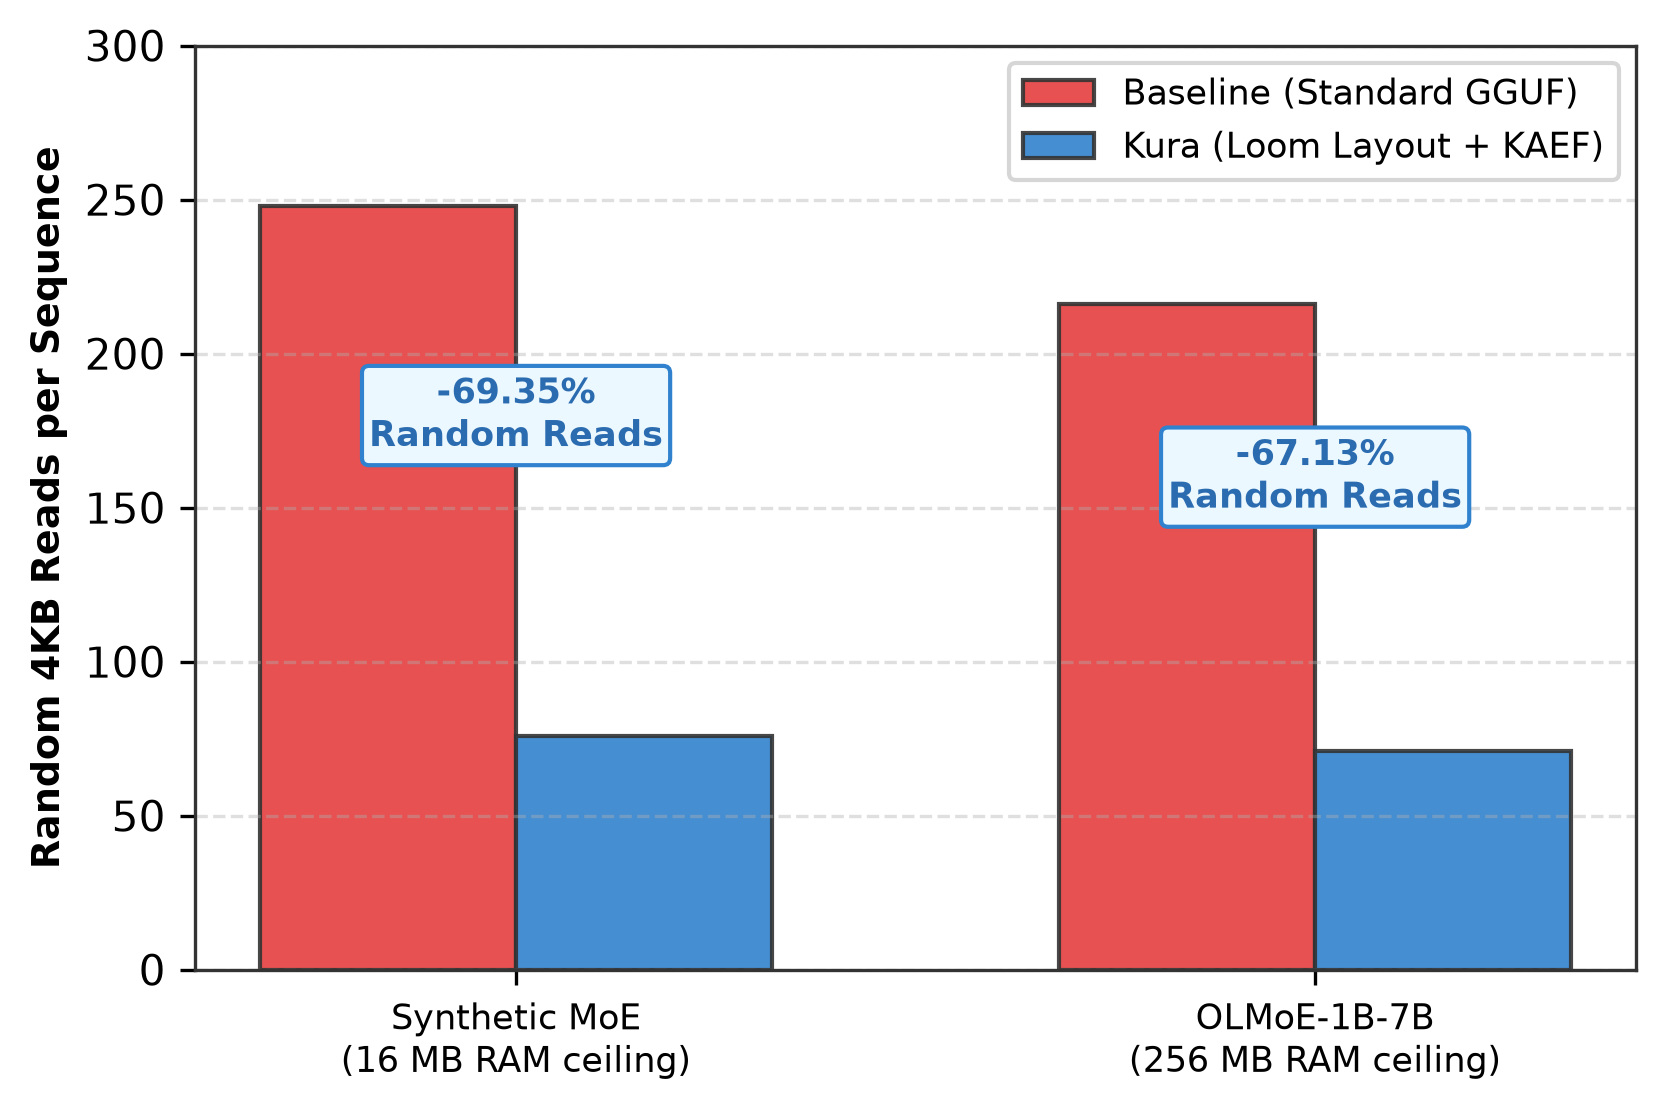
\includegraphics[width=\textwidth]{figures/fig2_random_read_reduction.png}
    \caption{Random NVMe reads under GGUF vs.\ Loom.}
    \label{fig:io_trace}
\end{subfigure}
\hfill
\begin{subfigure}[b]{0.48\textwidth}
    \centering
    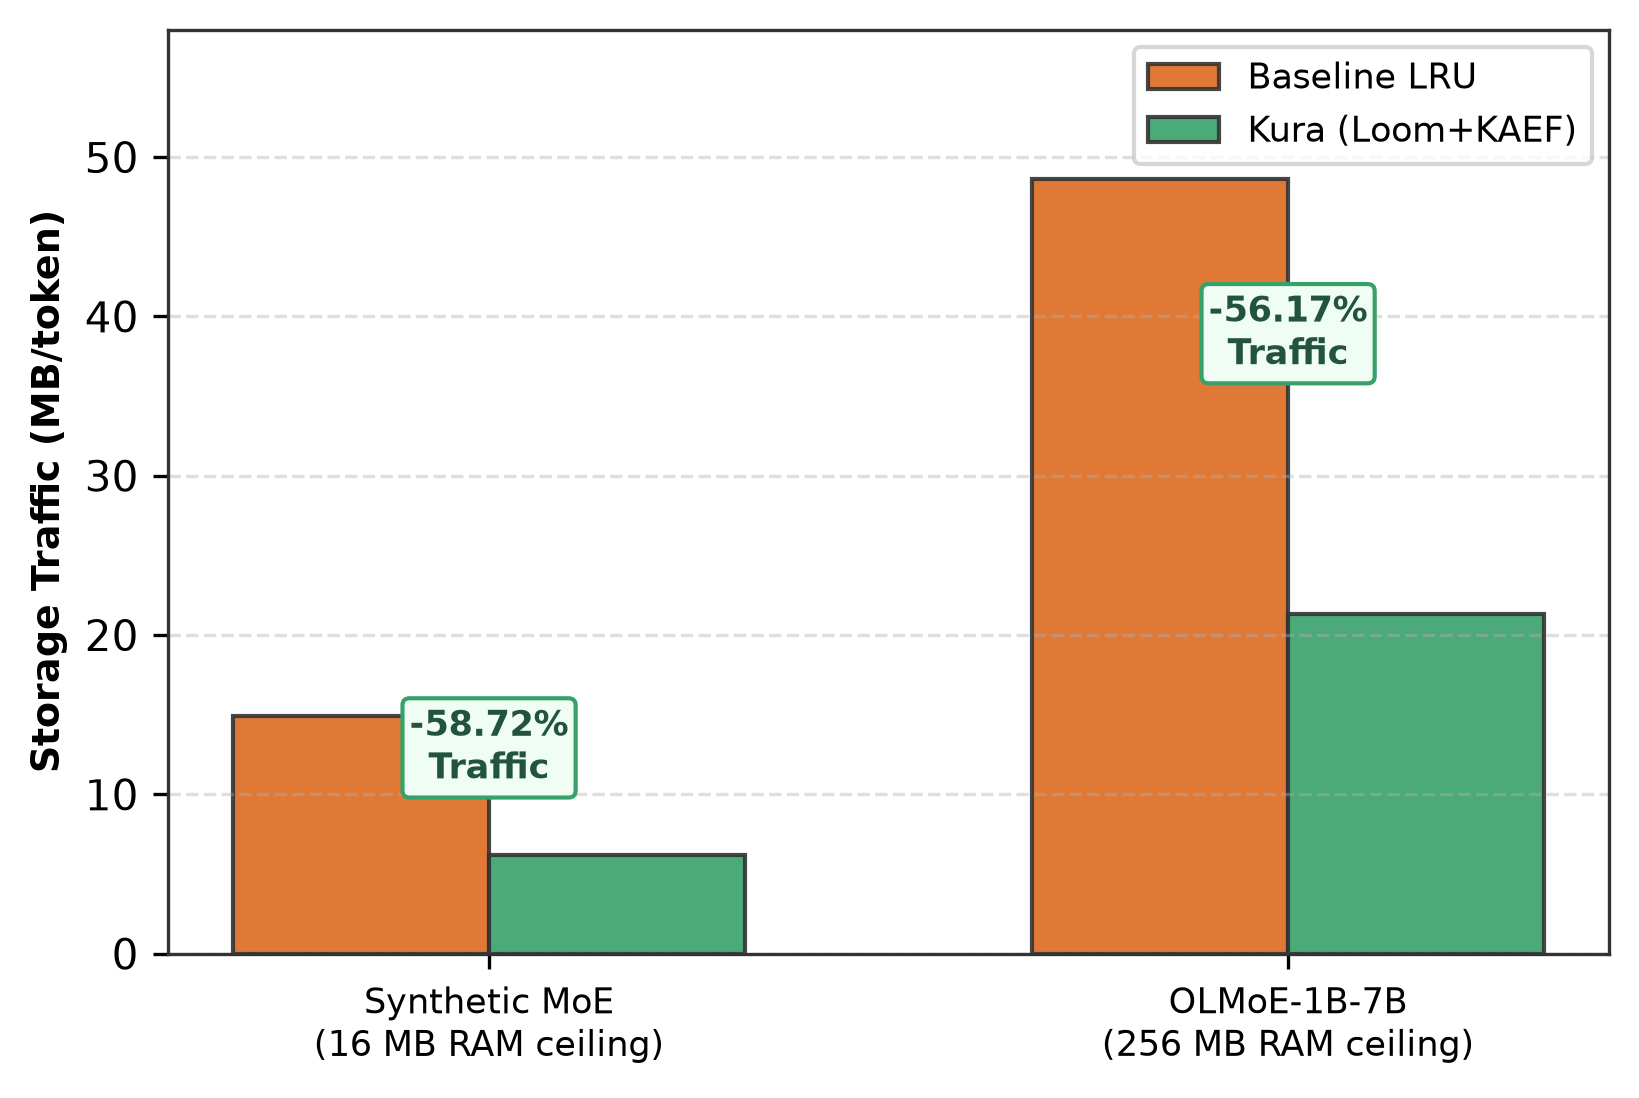
\includegraphics[width=\textwidth]{figures/fig3_storage_traffic.png}
    \caption{Storage traffic under constrained RAM budgets.}
    \label{fig:storage_traffic}
\end{subfigure}
\caption{Storage and I/O efficiency under Loom and KAEF. (a) Standard GGUF serial ordering forces scattered random 4\,KB reads across disk offsets, while Loom coalesces co-activated experts into contiguous physical extents, reducing random reads by $67.1\%$ to $69.4\%$. (b) Under severe memory scarcity, KAEF reduces storage traffic by $58.7\%$ under a 16\,MB RAM budget on Synthetic MoE ($10.4\times$ pressure) and by $56.2\%$ on OLMoE-1B-7B under a 256\,MB RAM budget ($4.8\times$ pressure).}
\label{fig:loom_eval}
\end{figure*}

While KAEF optimizes online memory residency decisions, the underlying physical transfer cost of non-resident experts remains fundamentally governed by NVMe hardware characteristics. Standard file formats (such as GGUF) store model tensors in sequential linear order:
\begin{equation}
    \mathcal{L}_{\text{standard}} = \left[ F_1^{(1)}, F_2^{(1)}, \dots, F_E^{(1)}, F_1^{(2)}, \dots, F_E^{(L)} \right]
\end{equation}
When the router selects experts $F_2^{(1)}$ and $F_{61}^{(1)}$, the disk controller must execute two geographically separated I/O operations across disk address spaces. \textsc{Loom} addresses this structural limitation by compiling physical storage layouts to align with empirical activation dynamics.

\subsection{Co-Activation Markov Graph Construction}
Loom operates as an offline compiler prior to runtime deployment. Given a representative calibration corpus $\mathcal{D}_{\text{calib}}$, Loom records the activation sequences of router selections across all layers.
For each layer $l$, Loom constructs an undirected weighted co-activation graph $\mathcal{G}^{(l)} = (\mathcal{V}^{(l)}, \mathcal{E}^{(l)}, \mathcal{W}^{(l)})$, where vertices $\mathcal{V}^{(l)} = \{1, \dots, E\}$ represent the individual experts. The edge weight $w_{ij}^{(l)} \in \mathcal{W}^{(l)}$ between expert $i$ and expert $j$ represents the empirical joint co-activation frequency:
\begin{equation}
    w_{ij}^{(l)} = \sum_{t=1}^{|\mathcal{D}_{\text{calib}}|} \mathbb{I}\left( i \in \mathcal{A}_t^{(l)} \land j \in \mathcal{A}_t^{(l)} \right)
\end{equation}
The resulting adjacency matrix $A^{(l)} \in \mathbb{R}^{E \times E}$ captures the spatial affinity of expert executions.

\subsection{Spectral Partitioning and Block Coalescing}
To map the high-dimensional affinity graph $\mathcal{G}^{(l)}$ onto a one-dimensional physical NVMe address space, Loom applies spectral graph partitioning~\citep{von2007tutorial}.
Let $D^{(l)} = \text{diag}\left(\sum_j w_{ij}^{(l)}\right)$ denote the degree matrix, and let $L_{\text{norm}}^{(l)} = I - (D^{(l)})^{-1/2} A^{(l)} (D^{(l)})^{-1/2}$ denote the normalized graph Laplacian.
Loom computes the Fiedler vector $v_2^{(l)}$—the eigenvector corresponding to the second-smallest eigenvalue of $L_{\text{norm}}^{(l)}$:
\begin{equation}
    L_{\text{norm}}^{(l)} v_2^{(l)} = \lambda_2 v_2^{(l)}
\end{equation}
The 1D ordering $\pi^{(l)}: \{1, \dots, E\} \to \{1, \dots, E\}$ is derived by sorting the elements of $v_2^{(l)}$:
\begin{equation}
    \pi^{(l)} = \text{argsort}\left( v_2^{(l)} \right)
\end{equation}
Sorting the continuous coordinates of the Fiedler vector yields a discrete permutation $\pi$ that serves as a standard spectral relaxation heuristic approximating the 1D minimum arrangement problem, ensuring that experts with high empirical co-activation frequencies are assigned adjacent permutation indices without claiming unconstrained discrete optimality.

\subsection{Contiguous NVMe Sidecar File Layout}
Using the optimized permutation $\pi^{(l)}$, Loom compiles a custom binary sidecar file (\texttt{.kura\_sidecar}).
Expert weights are grouped into super-blocks aligned to physical 128\,KB NVMe boundaries. When KAEF schedules the prefetch of expert $F_i^{(l)}$, Kura checks whether adjacent co-activated experts $F_{\pi(i)+1}^{(l)}$ in the Loom cluster have non-zero MEC values. If so, Kura issues a single coalesced sequential read request spanning both experts:
\begin{equation}
    \text{Request} = \left( \text{offset} = \text{Addr}\left(F_{\pi(i)}\right), \text{length} = 2 \cdot \mathcal{S}_{\text{exp}} \right)
\end{equation}
As shown in Figure~\ref{fig:io_trace}, this coalescing eliminates intermediate disk seeks and converts scattered random 4\,KB transfers into sustained, high-bandwidth sequential DMA bursts.
On OLMoE-1B-7B, Loom collapses random NVMe reads from 216 to 71 (a $67.1\%$ reduction), and on synthetic MoE benchmarks from 248 to 76 (a $69.3\%$ reduction).
